\section{Part 1C: Finding and measuring acoustic correlates of voicing}

\subsection{Before you start}

In this part of the lab we will be trying to identify and measure the acoustic correlates of the articulatory feature of \emph{voicing}. We will still be using \Praat{} to do the analysis and measurements, but we will now use a spreadsheet to collect the measurements and plot the data. In what follows, I am assuming the usage of \MSExcel{}\footnote{The figures were generated in an older version of \MSExcel{}, so it may not match the visual interface you will get when using the newer versions, but the functionality should be equivalent.}, but I assume any other spreadsheet program like \OpOff{} or \Gsheet{} will probably work as well with minimal modifications.

\subsection{Overview}

So far we have looked at the following consonants: [b], [d] and [g]. However, they constitute only half of the inventory for the English stop consonants. The other half, [p], [t] and [k] are remarkably close in articulatory terms to [b], [d] and [g] --- namely, they respectively share their place of articulation. In fact, the only difference between the two subsets is what phonologists call ``voicing''. The easiest way to grasp what ``voicing'' is is to say [pa] and [ba] with your index and middle fingers on your throat. Notice the difference? Your vocal chords vibrate more when you articulate the latter than when you articulate the former.

Locate the sound file \filefmat{thedot\_thetot.wav}, which contains the recording of a native speaker of English uttering the following two words in close succession: \emph{the dot, the tot}. Open this file in \Praat{} by clicking on \softmenu{Read} $>$ \softmenu{Read from file\ldots}) and once the file is in the \softmenu{Objects} window, click on it and press the \softmenu{View \& Edit} button to open the sound editor window. It should look like figure~\ref{step1VOT}.

\begin{figure}[!tbp]
\caption{\Praat{} -- Spectrogram of \emph{the dot, the tot}}
\label{step1VOT}
	\begin{center}
		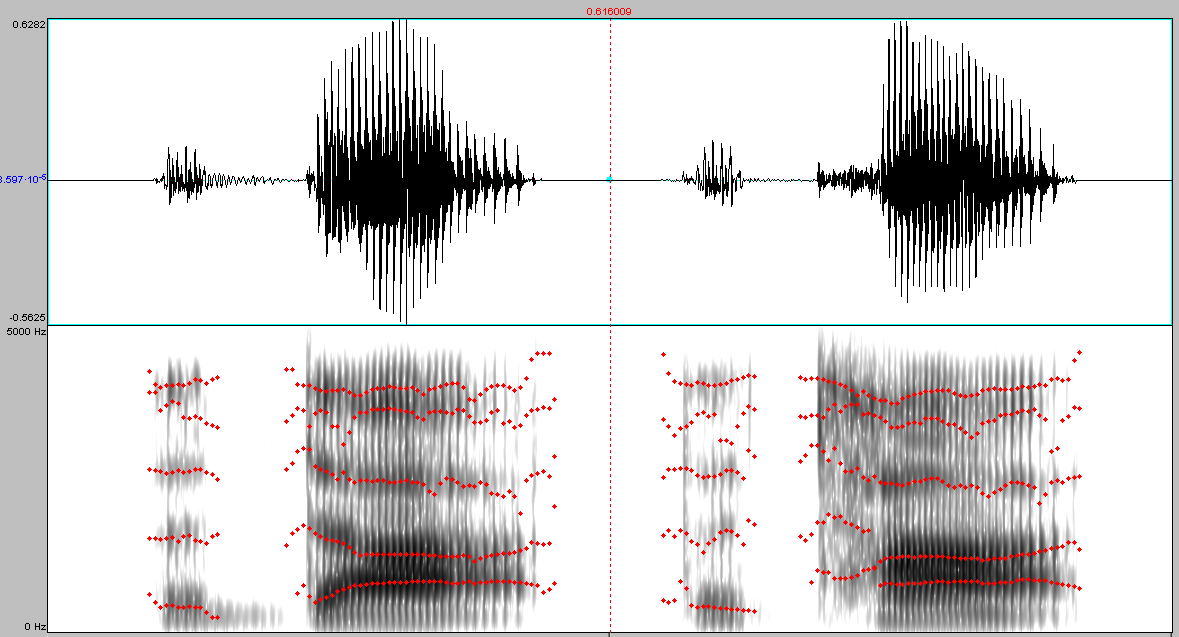
\includegraphics[width=0.8\textwidth]{./figures/Part-C-VOT-thedotthetot1}
	\end{center}
\end{figure}

\paragraph{Write--up:} Can you see the difference between the voiced (\emph{dot}) and unvoiced (\emph{tot}) consonants? What is it? (Tip: you should look at the waveform as well, since it is also informative). Once you have figured this one out and written it up, move on.

\paragraph{Write--up:} The difference you observed between the two consonants ([d] and [t]) is called the ``burst'', and it is the flow of air following the release of the stop. Notice how it has energy spread over a wide range of frequencies (the big relatively uniform grayish area before the vowel), and how it is especially salient for [t]; [d] has barely any visible burst on the display. The time between the onset of the burst (i.e., the stop release) and the onset of voicing (in this case, the vowel) receives the name of Voice Onset Time, or simply VOT. Since this seems to be the acoustic cue that sets voiced and unvoiced stop consonants apart, we are going to be measuring it.

Your task now is to open the files containing the recordings of a different native speaker of American English saying the two words (\emph{the dot, the tot}) and measure the VOT of both consonants.

Here's how you do it. First, zoom in in the \emph{the tot} utterance, as shown in figure~\ref{step2VOT}. Now, try to find and select the chunk of time between the onset of the burst and the onset of the vowel, as shown in figure~\ref{step3VOT}. 

\begin{figure}[!tbp]
\caption{\Praat{} -- Spectrogram of \emph{the dot, the tot} -- zooming in}
\label{step2VOT}
	\begin{center}
		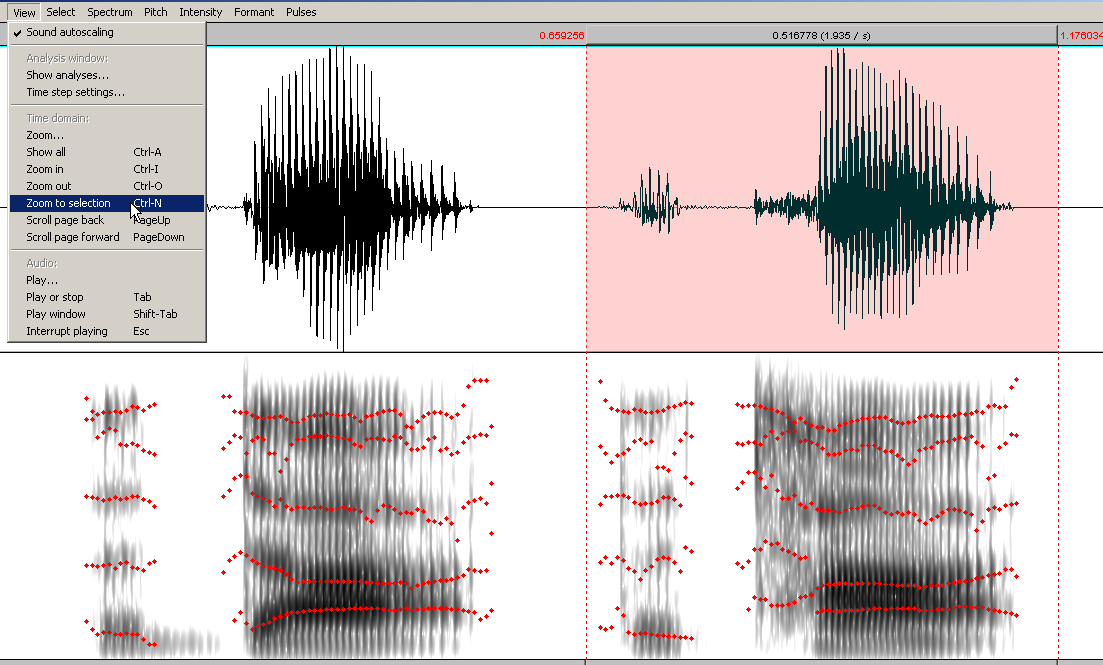
\includegraphics[width=0.8\textwidth]{./figures/Part-C-VOT-thedotthetot-zoom}
	\end{center}
\end{figure}

\begin{figure}[!tbp]
\caption{\Praat{} -- Spectrogram of \emph{the dot, the tot} -- Measuring the VOT of [t]}
\label{step3VOT}
	\begin{center}
		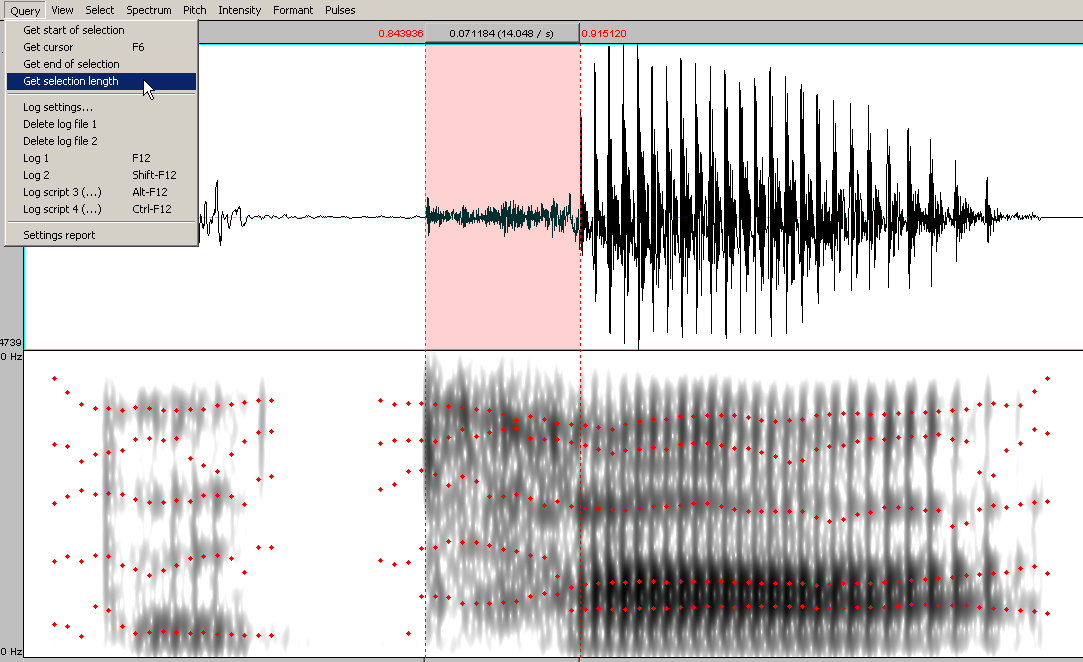
\includegraphics[width=0.8\textwidth]{./figures/Part-C-VOT-thedotthetot-measuring-unvoiced}
	\end{center}
\end{figure}

Once you are confident in your selection, go to \softmenu{Query} $>$ \softmenu{Get selection length}, and copy and paste the value you get into a spreadsheet, as shown in figure~\ref{step4VOT} --- notice the little trick to transform the measurements from seconds to miliseconds.

\begin{figure}[!tbp]
\caption{\MSExcel{} -- Saving your measurements}
\label{step4VOT}
	\begin{center}
		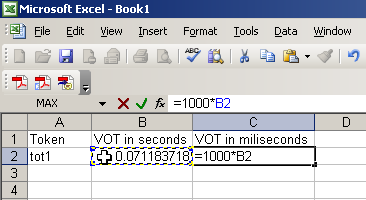
\includegraphics[width=0.8\textwidth]{./figures/Part-C-VOT-thedotthetot-Excel01}
	\end{center}
\end{figure}

Now you should try to measure the VOT of [d]. Unzoom from where you are (\softmenu{View} $>$ \softmenu{Show all}) and zoom in on the first utterance. As you can see in figure~\ref{step5VOT}, the VOT is much smaller than the one for [t]. In fact, it is very possible you will need to zoom in some more in your own recordings to see the burst at all, since the quality of the recording will probably not be as good. Once you are satisfied with your selection, get the values into the spreadsheet.

\begin{figure}[!tbp]
\caption{\Praat{} -- Spectrogram of \emph{the dot, the tot} -- Measuring the VOT of [d]}
\label{step5VOT}
	\begin{center}
		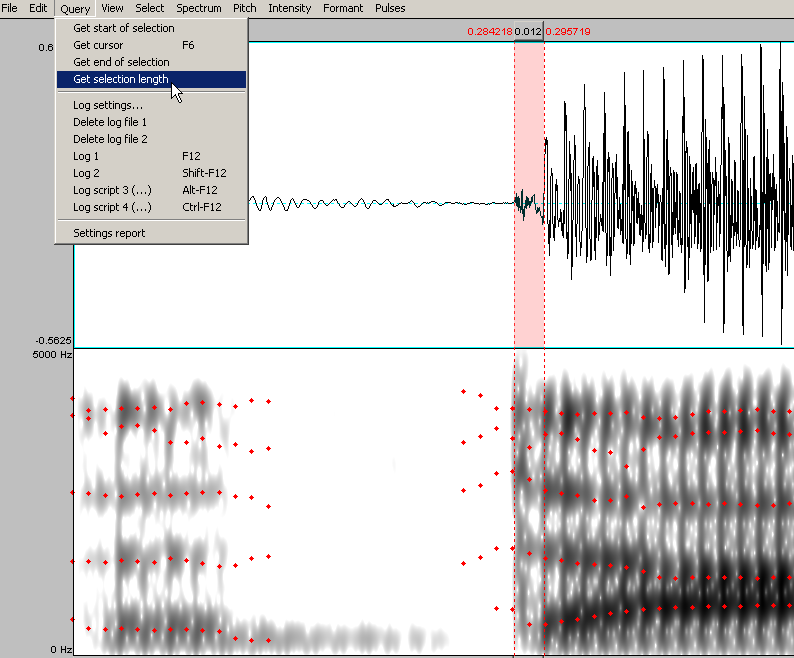
\includegraphics[width=0.8\textwidth]{./figures/Part-C-VOT-thedotthetot-measuring-voiced}
	\end{center}
\end{figure}
 
Try to get the values of the 15 repetitions files. By the end, your spreadsheet should look something like figure~\ref{step6VOT}.

\begin{figure}[!tbp]
\caption{\MSExcel{} -- What your spreadsheet should look like}
\label{step6VOT}
	\begin{center}
		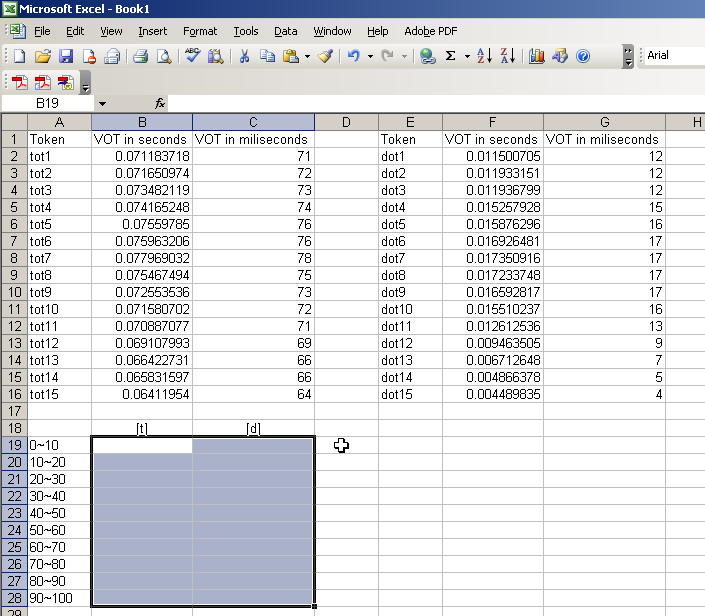
\includegraphics[width=0.8\textwidth]{./figures/Part-C-VOT-thedotthetot-Excel03}
	\end{center}
\end{figure}

\paragraph{Write--up:} Notice the time--bins (0--10, 10--20, \dots{}, 90--100) on the bottom of the spreadsheet, with two empty columns, one under [t] and one under [d]. Your task now is to populate these columns with the counts of how many observations you had in each time--bin. For instance, if you had two [t] VOTs falling into the bin 60--70ms, then you should input ``2'' on the column ``[t]'' next to the bin ``60--70''. Once you are done, you should plot a bar graph of the data you collected, with the time--bins as the x--axis and the counts on the y--axis, as shown in figure~\ref{step7VOT}. What can you conclude from your graph? Does VOT constitute a good acoustic cue to differentiate voiced and unvoiced stops?

\begin{figure}[!tbp]
\caption{\MSExcel{} -- Plotting the VOT bar graph}
\label{step7VOT}
	\begin{center}
		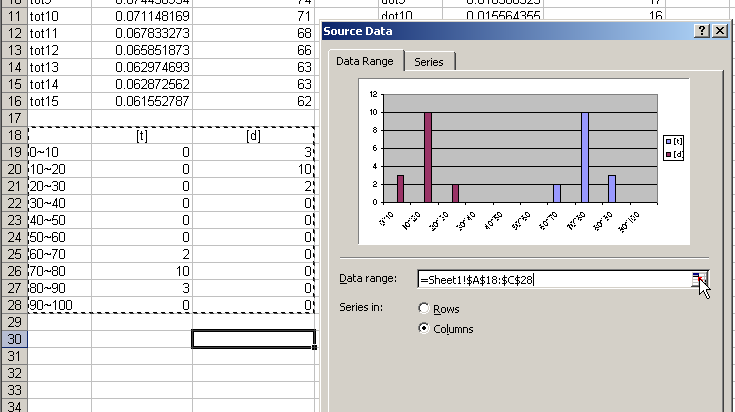
\includegraphics[width=0.8\textwidth]{./figures/Part-C-VOT-thedotthetot-Excel04}
	\end{center}
\end{figure}
 
\subsection{What you need to write up}

All the parts marked as \emph{Write--up} in the instructions above should be incorporated in your lab write--up, together with the plots they require. Try to articulate your impressions and results the best you can, in full coherent sentences (no bullets, please).


